\documentclass[10pt]{article}
\usepackage[paperwidth=190mm,paperheight=56mm,margin=2mm]{geometry}
\usepackage{fontspec}
\usepackage{tikz}
\usetikzlibrary{positioning}
\setmainfont{DejaVu Sans}
\pagestyle{empty}

\begin{document}
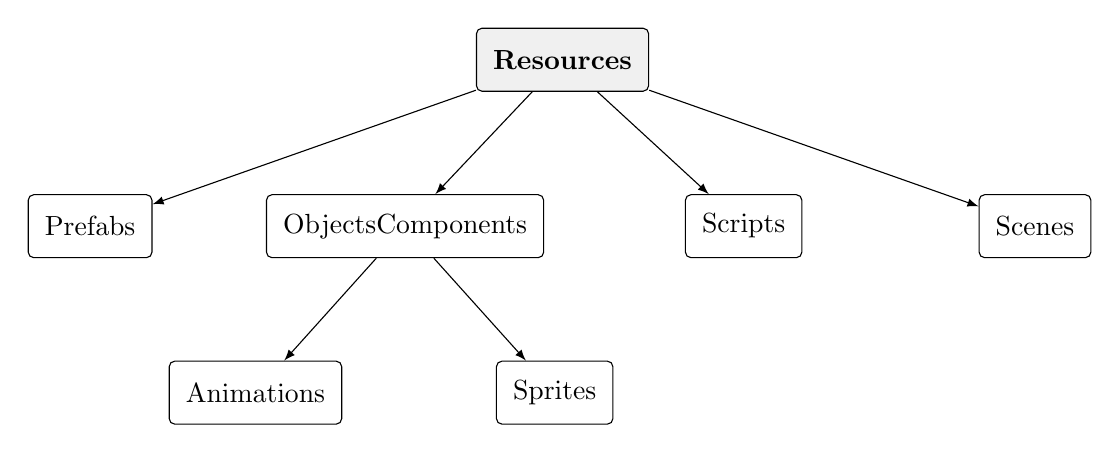
\begin{tikzpicture}[
  box/.style={
    draw,
    rounded corners=2pt,
    align=center,
    font=\normalsize,
    minimum height=8mm,
    inner xsep=6pt,
    fill=white
  },
  root/.style={box, fill=gray!12, font=\bfseries\normalsize},
  line/.style={draw, -latex}
]
\node[root] (resources) {Resources};
\node[box, below=13mm of resources, xshift=-60mm] (prefabs) {Prefabs};
\node[box, below=13mm of resources, xshift=-20mm] (components) {ObjectsComponents};
\node[box, below=13mm of resources, xshift=23mm] (scripts) {Scripts};
\node[box, below=13mm of resources, xshift=60mm] (scenes) {Scenes};

\node[box, below=13mm of components, xshift=-19mm] (animations) {Animations};
\node[box, below=13mm of components, xshift=19mm] (sprites) {Sprites};

\draw[line] (resources) -- (prefabs);
\draw[line] (resources) -- (components);
\draw[line] (resources) -- (scripts);
\draw[line] (resources) -- (scenes);
\draw[line] (components) -- (animations);
\draw[line] (components) -- (sprites);
\end{tikzpicture}
\end{document}
